\documentclass[twocolumn,10pt]{article}
\usepackage[a4paper, top=1.0in, bottom=1.0in, left=0.85in, right=0.85in]{geometry}

\usepackage{graphicx}
\usepackage{algorithm}  
\usepackage{algorithmicx}  
\usepackage{algpseudocode}  
\usepackage{amsmath}
\usepackage{url}

\renewcommand{\algorithmicrequire}{\textbf{Input:}}  
\renewcommand{\algorithmicensure}{\textbf{Output:}}  
\graphicspath{{figure/}}

\begin{document}
	
\date{November 17th, 2016}

\title{\bf Song Paper}

\author{
	Meng Li, 201620728  
	\\ Supervisor: Yasushi Shinjo
}

\maketitle

\section{Introduction}
Cao ni da ye\cite{dong2016aggregate}

\begin{figure}[t]
	\centering
	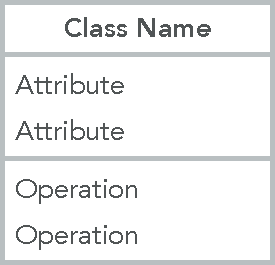
\includegraphics[scale=0.5]{1}
	\caption{Entities in the Web service.}
\end{figure}

\begin{table}[tbp]
	\centering  
	\begin{tabular}{lll}  
		\hline
		Column &Data Type & Introduction\\ 
		\hline  
		sid &String & Physical unique identifier\\
		content & String & JSON String of object\\ 
		object & String & Name of object\\
		count & Integer16 & Count of sync time\\
		resend & Boolean &Necessity of resending data \\
		sendtime & Date & Data send time\\
		\hline
	\end{tabular}
	\caption{Columns of sender table}
\end{table}

\bibliographystyle{unsrt}
{
	\footnotesize
	\bibliography{ref}
}

\end{document}
